\documentclass[11pt]{article}
\usepackage{graphicx}
\usepackage{placeins}


% acronyms for text or math mode
\newcommand {\ccast} {\mbox{\small CCAST}}
\newcommand {\cris} {\mbox{\small CrIS}}

\newcommand {\airs} {\mbox{\small AIRS}}
\newcommand {\iasi} {\mbox{\small IASI}}
\newcommand {\idps} {\mbox{\small IDPS}}
\newcommand {\nasa} {\mbox{\small NASA}}
\newcommand {\noaa} {\mbox{\small NOAA}}
\newcommand {\nstar} {\mbox{\small STAR}}
\newcommand {\umbc} {\mbox{\small UMBC}}
\newcommand {\uw}   {\mbox{\small UW}}

\newcommand {\fft}  {\mbox{\small FFT}}
\newcommand {\ifft} {\mbox{\small IFFT}}
\newcommand {\fir}  {\mbox{\small FIR}}
\newcommand {\fov}  {\mbox{\small FOV}}
\newcommand {\for}  {\mbox{\small FOR}}
\newcommand {\ict}  {\mbox{\small ICT}}
\newcommand {\ils}  {\mbox{\small ILS}}
\newcommand {\igm}  {\mbox{\small IGM}}
\newcommand {\opd}  {\mbox{\small OPD}}
\newcommand {\rms}  {\mbox{\small RMS}}
\newcommand {\zpd}  {\mbox{\small ZPD}}
\newcommand {\ppm}  {\mbox{\small PPM}}
\newcommand {\srf}  {\mbox{\small SRF}}
\newcommand {\sdr}  {\mbox{\small SDR}}

\newcommand {\ES} {\mbox{\small ES}}
\newcommand {\SP} {\mbox{\small SP}}
\newcommand {\IT} {\mbox{\small IT}}
\newcommand {\SA} {\mbox{\small SA}}

\newcommand {\ET} {\mbox{\small ET}}
\newcommand {\FT} {\mbox{\small FT}}

\newcommand {\wn} {\mbox{cm$^{-1}$}}

% abbreviations, mainly for math mode
\newcommand {\real} {\mbox{real}}
\newcommand {\imag} {\mbox{imag}}
\newcommand {\atan} {\mbox{atan}}
\newcommand {\obs}  {\mbox{obs}}
\newcommand {\calc} {\mbox{calc}}
\newcommand {\sinc} {\mbox{sinc}}
\newcommand {\psinc} {\mbox{psinc}}
\newcommand {\std} {\mbox{std}}

% symbols, for math mode only
\newcommand {\lmax} {L_{\mbox{\tiny max}}}
\newcommand {\vmax} {V_{\mbox{\tiny max}}}

\newcommand {\tauobs} {\tau_{\mbox{\tiny obs}}}
\newcommand {\taucal} {\tau_{\mbox{\tiny calc}}}
\newcommand {\Vdc}  {V_{\mbox{\tiny DC}}}

\newcommand {\rIT} {r_{\mbox{\tiny\textsc{ict}}}}
\newcommand {\rES} {r_{\mbox{\tiny\textsc{es}}}}
\newcommand {\robs} {r_{\mbox{\tiny obs}}}

\newcommand {\rITobs} {r_{\mbox{\tiny\textsc{ict}}}^{\mbox{\tiny obs}}}
\newcommand {\rITcal} {r_{\mbox{\tiny\textsc{ict}}}^{\mbox{\tiny cal}}}

\newcommand {\ITmean} {\langle\mbox{\small IT}\rangle}
\newcommand {\SPmean} {\langle\mbox{\small SP}\rangle}


\title{AIRS Deconvolution and Translation \\
  from the AIRS to CrIS IR Sounders \\
  \vspace{3mm}
  {****} DRAFT {****}\\
}

\author{Howard E.~Motteler \\
  L.~Larrabee Strow \\
  \\
  UMBC Atmospheric Spectroscopy Lab \\
  Joint Center for Earth Systems Technology \\
}

\date{\today}
\begin{document}
\maketitle

\section{Introduction}

Upwelling infrared radiation as measured by the {\airs} \cite{airs1}
and {\cris} \cite{cris1,cris2} sounders is a significant part of the
long term climate record.  We would like to treat this as a single
data set and often want to compare radiances, for example in the
analysis of simultaneous nadir overpasses (SNOs) for sounder
calibration or validation.  However the instruments have different
spectral resolutions, channel response functions, and band spans.
As a step in addressing this problem we consider the translation of
channel radiances from {\airs} to standard resolution {\cris}.

Translation from {\airs} to {\cris} involves more that basic
resampling.  {\airs} is a grating spectrometer with a distinct
response function for each channel determined by the focal plane
geometery, while {\cris} is a Michaelson interferometer with a sinc
response function, after calibration and corrections.  In section
\ref{decon} we show how to take advantage of our detailed knowledge
of the {\airs} spectral response functions (SRFs) and their overlap
to deconvolve channel radiances to a resolution-enhanced
intermediate representation, typically a $0.1$~\wn\ grid, the
approximate resolution of the tabulated {\airs} SRFs.  

This intermediate representation can then be reconvolved, for
example to an idealized grating instrument with a generalized
Gaussian response function or to the {\cris} user grid with a sinc
basis.  Section \ref{airs2cris} gives details and validation tests
for the {\airs} to {\cris} translation.  In section \ref{statfix} 
we consider alternate translations, including conventional
interpolation and direct regression from {\airs} to {\cris}.
Section \ref{appcon} gives some applications and conclusions.

\FloatBarrier
\section{AIRS Deconvolution}
\label{decon}

The {\airs} spectral response functions model channel response as a
function of frequency and associate channels with nominal center
frequencies.  Each {\airs} channel $i$ has an associated spectral
response function or {\srf} $\sigma_i(v)$ such that the channel
radiance $c_i = \int \sigma_i(v)r(v)\,dv$, where $r$ is radiance at
frequency $v$.  The center or peak of $\sigma_i$ is the nominal
channel frequency.

\begin{figure} % source plot_SRF2.m
  \centering
  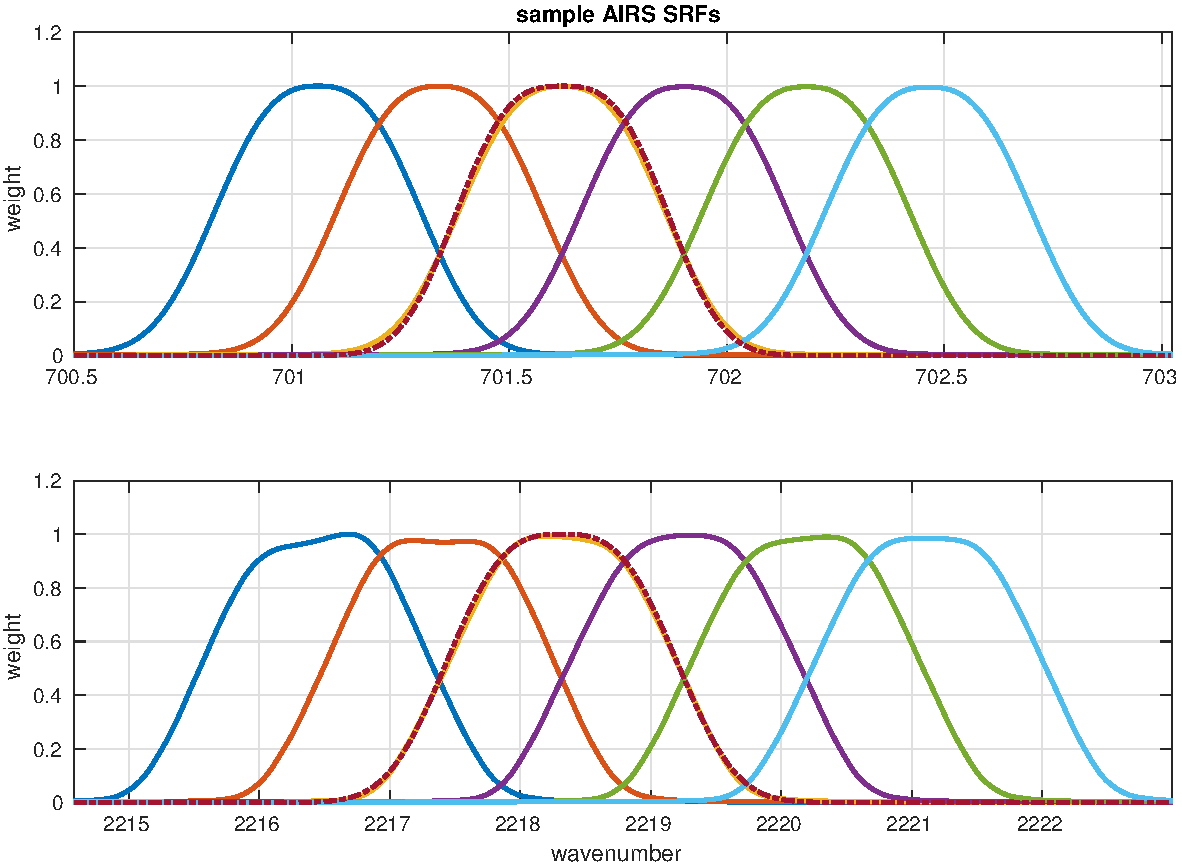
\includegraphics[height=7.5cm]{figures/airs_sample_srfs.pdf}
  \caption{sample {\airs} spectral response functions from the low
    and high ends of the band.   The dashed line is a generalized
    Gaussian function.}
  \label{srfs1}
\end{figure}

\begin{figure} % source plot_SRF2.m
  \centering
  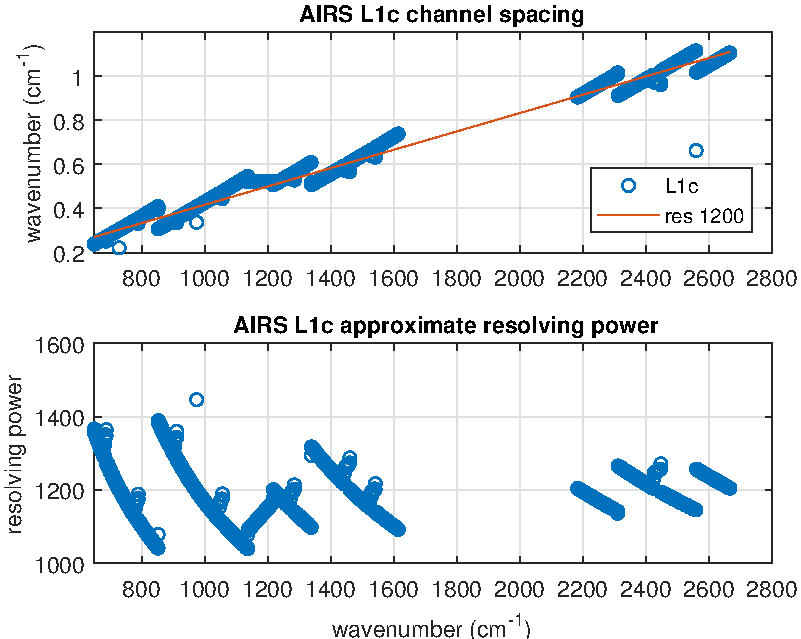
\includegraphics[height=7.5cm]{figures/airs_L1c_res.pdf}
  \caption{{\airs} L1c channel spacing and derived resolving
    power.}
  \label{chan1}
\end{figure}

Figure \ref{srfs1} shows typical {\airs} SRFs from the low and high
ends of the band.  Note the significant overlap in the wings.  This
can allow for a deconvolution to recover resolution beyond that of
the response functions considered individually.  The SRFs are not
necessarily symmetrical, especially at the high end of the band.
The dashed line on top of the third SRF is a fit of a generalized
Gaussian, which we consider in more detail later in this section.
Figure \ref{chan1} shows channel spacing and resolving power for the
{\airs} L1c channel set \cite{airs1c}.  The variable channel spacing
and resolving power are due to the modular structure of the focal
plane.  Although not entirely regular---that is, not a simple
function of frequency---the L1c channel set is more regular than the
L1b channel set from which it is derived, and we mainly consider the
L1c set here.

Suppose we have $n$ channels and a frequency grid $\vec v$ of $k$
points spanning the union of the domains of the functions
$\sigma_i$.  The grid step size for our applications is often 0.0025
{\wn}, the kcarta resolution \cite{kcarta1}.  Let $S_k$ be an
$n\times k$ array such that $s_{i,j} = \sigma_i(v_j)/w_i$, where
$w_i = \sum_j \sigma_i(v_j)$, that is where row $i$ is $\sigma_i(v)$
tabulated at the grid $\vec v$ and normalized so the row sum is 1.
If the channel centers are in increasing order $S_k$ is banded, and
if they are not too close (as is the case for a few of the L1b
channels) the rows are linearly independent.  $S_k$ is a linear
transform whose domain is radiance at the grid $\vec v$ and whose
range is channel radiances.  If $r$ is radiance at the grid $\vec
v$, then $c = S_k r$ gives a good approximation of the channel
radiances $c_i = \int\sigma_i(v)r(v)\,dv$.  In practice this is how
we convolve kcarta or other high resolution calculated radiances to
get {\airs} channel radiances, for example for reference truth or
``true {\airs}'' for the tests shown here.

% We construct $S_k$ either explicitly or implicitly from the
% {\airs} {\srf} tabulations.  The matrix $S_k$ in the former case
% is large but manageable with a banded or sparse representation.

For the {\airs} to {\cris} and other translations we are mainly
interested in the transform $S_b$ for {\srf}s at an intermediate
resolution, typically 0.1 {\wn}.  This is the approximate resolution
of the {\srf} measurements and convenient for reconvolution to the
{\cris} user grid.  So let $\vec v_b = v_1,v_2,\ldots,v_m$ be a $0.1
\wn$ grid spanning the domains of the functions $\sigma_i$.  Similar
to $S_k$, let $S_b$ be an $n\times m$ array where row $i$ is
$\sigma_i(v)$ tabulated at the $\vec v_b$ grid, with rows normalized
to~1.  If $r$ is radiance at the $\vec v_b$ grid, then $c = S_b r$
is still a reasonable approximation of $\int\sigma_i(v)r(v)\,dv$.

For our application we want to start with $c$ and find $r$, that is
to deconvolve $c$ by solving $S_b r = c$ for $r$.  Since $m < k$,
the system is underdetermined, but we can take $r$ as $r_0 =
S_b^{-1} c$ where $S_b^{-1}$ is the Moore-Penrose pseudoinverse
\cite{pinv} of $S_b$.  This has the key property of finding $r_0$
such that $||r_0||_2 \le ||r_j||_2$ for all $r_j$ satisfying $S_b
r_j = c$.  The condition number for $S_b$ built from the L1c
channels is $||S_b||_2||S_b^{-1}||_2 = 115$, which is acceptable.

Although our main goal is to reconvolve the $0.1~\wn$ intermediate
representation to the {\cris} or other user grids, we first compare
the deconvolved radiances with reference truth from a direct
convolution to intermediate grid.  The choice of response functions
for this direct convolution is not obvious, since the deconvolution
is undoing---at least to some extent---the effects of the {\airs}
SRF convolutions.  We use a generalized Gaussian of the form
\[w = \exp\left(-\left(\frac{(x - v_0)^2}{2c^2}\right)^{1.5}\right) \]
where $c=\fwhm / 2.355$ and $v_0$ is the desired channel center.
The exponent $1.5$ was chosen to give an approximate match to
{\airs} SRFs with the same {\fwhm} and channel centers, though
without the fine structure and variation of the latter.  Figure
\ref{srfs1} shows two such functions paired with {\airs} SRFs with
the same {\fwhm} and centers.  We used this function for the
0.1~\wn\ intermediate grid with ${\fwhm} = v_i / 2000$ where $v_i$
are the grid frequencies.  This represents a hypothetical grating
spectrometer with a resolving power of 2000, oversampled to the
0.1~\wn\ grid.

% We also tried the generalized Gaussian with a fixed \fwhm\ for
% values $0.4$, $0.6$, and $0.8$ and a sinc basis with a spacing of
% $0.2$~\wn, all of which gave larger residuals.  The residual was
% roughly minimized for the resolving power of 2000 shown here.

\begin{figure} % source decon_test1.m 
  \centering
  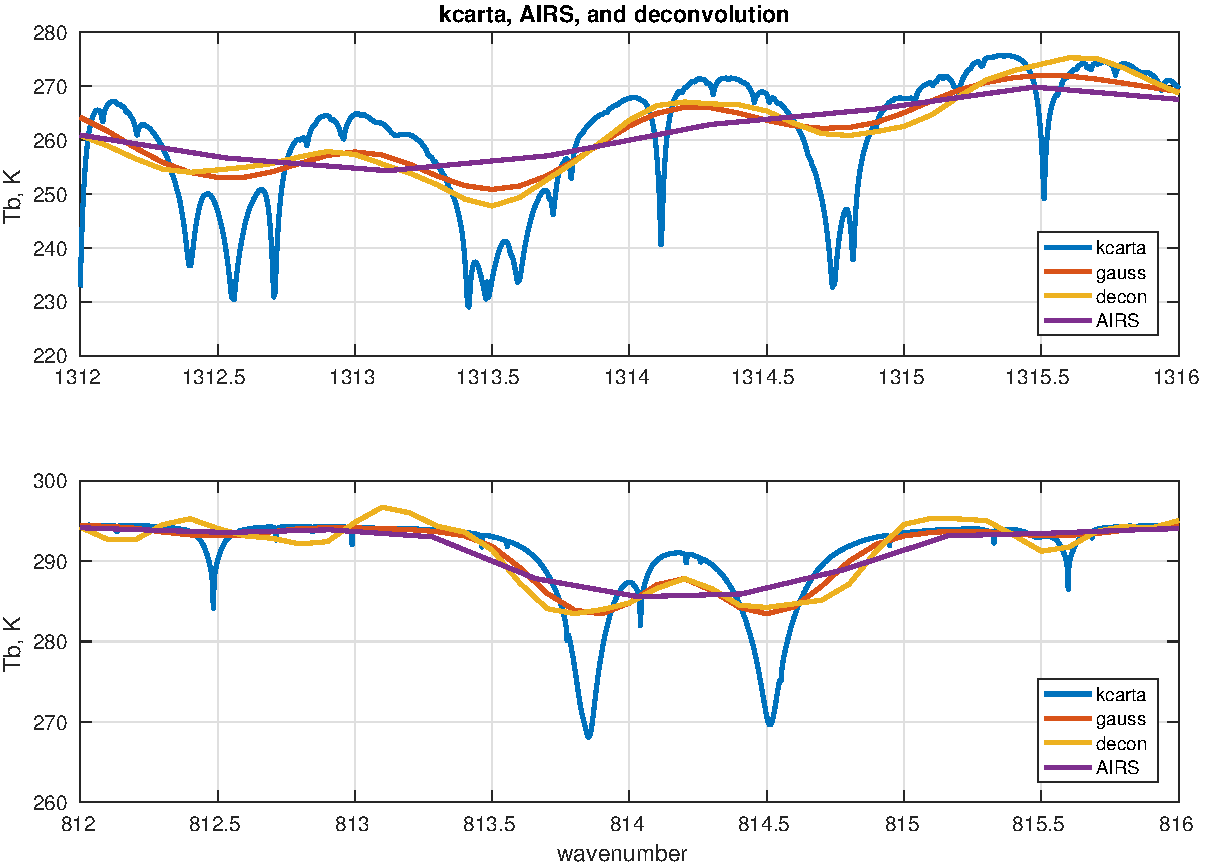
\includegraphics[height=7.5cm]{figures/airs_decon_zoom.pdf}
  \caption{details from fitting profile 1 for kcarta, direct
    convolution to the $0.1$~\wn\ grid (``gauss''), deconvolved
    {\airs}, and true {\airs}.}
  \label{dzoom}
\end{figure}

\begin{figure} % source decon_test1.m
  \centering
  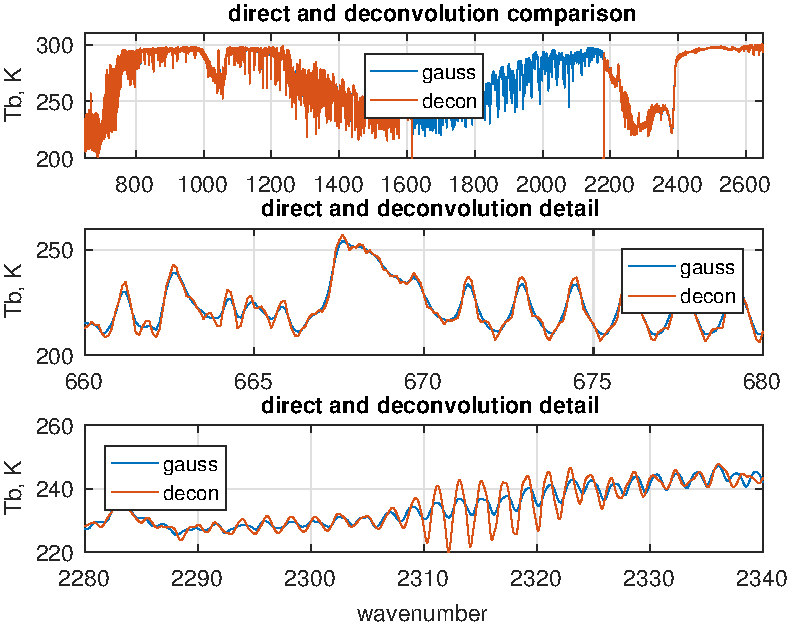
\includegraphics[height=7.5cm]{figures/airs_decon_spec.pdf}
  \caption{spectra from fitting profile 1 for direct convolution to
    the $0.1$~\wn\ grid (``gauss'') and deconvolved {\airs}}
  \label{dspec}
\end{figure}

% \begin{figure} % source decon_test1.m
%   \centering
%   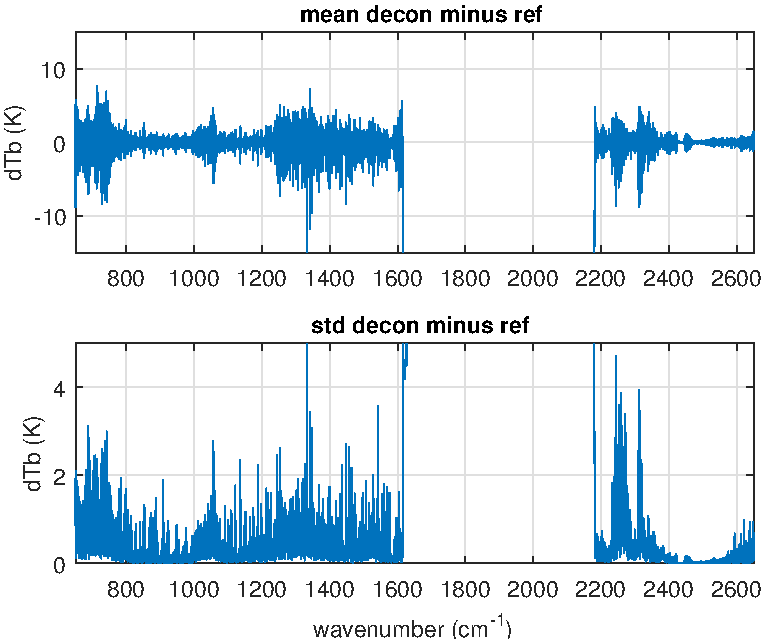
\includegraphics[height=7.5cm]{figures/airs_decon_diff.pdf}
%   \caption{mean and standard deviation over the 49 fitting profiles
%     for the L1c deconvolution minus direct convolution to the
%     $0.1$~\wn\ intermediate grid.  The residuals are too large to use
%     the deconvolved radiances directly.}
%   \label{ddiff}
% \end{figure}

The {\airs} deconvolution gives a modest resolution enhancement, at
the cost of added artifacts and noise.  Figure \ref{dzoom} shows
details of kcarta, direct convolution to the $0.1$~\wn\ grid
(``gauss''), deconvolution, and AIRS spectra for fitting profile~1
\cite{sarta1,sarta2}.  In the first subplot we see the deconvolution
is capturing some of the fine structure in the kcarta data that is
present in the direct convolution but not in the AIRS data.  In the
second subplot we see the deconvolution (and direct convolution)
resolving a pair of close lines that are not resolved at the {\airs}
L1c resolution.  But we also see some ringing that is not present in
the direct convolution.  Figure \ref{dspec} shows the full spectra
from fitting profile~1, along with sample details from the low and
high ends of the band, for the deconvolution and direct convolution
to the intermediate grid.  In the details we see some overshoot and
ringing in the deconvolution.  But we do not propose using the
deconvolved radiances directly, they are an intermediate step in
reconvolution to a lower resolution.

% Figure \ref{ddiff} shows the mean and standard deviation of the
% difference of the deconvolved minus the directly convolved radiances
% for all 49 fitting profiles.  The residuals are large but mainly
% significant for understanding limitations of the deconvolution.

% The residuals can be reduced dramatically by reconvolving the
% $0.1$~\wn\ intermediate grid to a lower resolution.  We consider
% this for convolution to the {\cris} user grid in the next section.

\begin{figure} % source plot_Binv.m
  \centering
  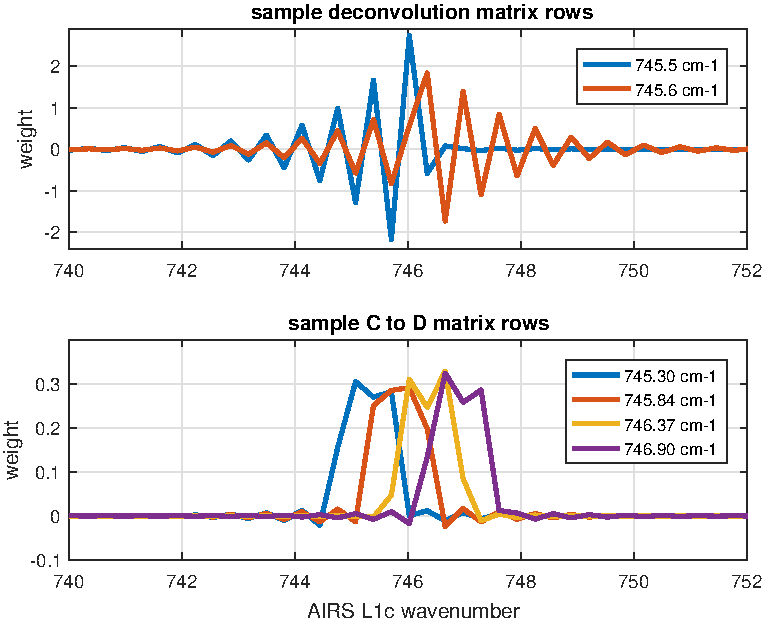
\includegraphics[height=7.5cm]{figures/airs_decon_basis.pdf}
  \caption{sample adjacent rows for the deconvolution and L1c to L1d
    transforms}
  \label{dbasis}
\end{figure}

Figure \ref{dbasis} shows a pair of typical adjacent rows of the
deconvolution matrix $S_b^{-1}$\, in the first subplot.  Row $i$ of
$S_b^{-1}$ is the weights applied to L1c channel radiances to
synthesize the deconvolved radiance $r_i$ at the intermediate grid
frequency $v_i$.  The oscillation simply means we are taking the
closest AIRS channel, subtracting weighted values for channels $\pm
1$ step away, adding weighted values for channels $\pm 2$ steps
away, and so on, with the weights decreasing quickly as we move away
from $v_i$, with eight to ten L1c channels making a significant
contribution to each deconvolution grid point.

The second subplot shows four adjacent rows of the matrix 
$S_d \cdot S_b^{-1}$, which takes L1c to L1d channel radiances.
(The L1d radiances are discussed in a later section; here they are
of interest mainly as a typical reconvolution.)  Both matrices are
banded but the bands are narrower in the second, with three to five
L1c channels contributing significantly to each L1d channel.  
The range of influence is significant since for example we may want
to see which L1d channels are derived in part from the subset of
synthetic L1c channels.

\FloatBarrier
\section{AIRS to CrIS translation}
\label{airs2cris}

% general setup from prev section:

For the tests here we start with a set of atmospheric profiles and
calculate upwelling radiance at a 0.0025 {\wn} grid with kcarta.
This is convolved with SRFs for the {\airs} L1c channel set to get
{\airs} reference truth, which we refer to as ``true {\airs}''.
Depending on the test we may also convolve the 0.0025 {\wn}
radiances with {\cris} or other SRFs to get ``true {\cris}'' or
other reference truth.  

For the {\cris} standard resolution mode the channel spacing is
$0.625$ {\wn} for the LW, 1.25~{\wn} for the MW, and 2.5~{\wn} for
the SW bands.  The first step in the {\airs} L1c to {\cris}
translation is to deconvolve the {\airs} channel radiances to the
0.1~{\wn} intermediate grid, the nominal {\airs} SRF resolution.
Then for each {\cris} band, we

\begin{itemize}
  \item find the {\airs} and {\cris} band intersection

  \item apply a bandpass filter to the deconvolved {\airs} radiances
    to restrict them to the intersection, with a rolloff outside the
    intersection

  \item reconvolve the filtered spectra to the {\cris} user grid

\end{itemize}

Translations are validated by comparison with calculated reference
truth.  For the results presented in this section we start with 49
fitting profiles spanning a significant range of atmospheric
conditions \cite{sarta1,sarta2}.  Upwelling radiance is calculated
at a 0.0025 {\wn} grid with kcarta \cite{kcarta1} over a band
spanning the {\airs} and {\cris} response functions.  ``True
{\airs}'' is calculated by convolving the kcarta radiances with
{\airs} SRFs, and ``true {\cris}'' by convolving kcarta radiances to
a sinc basis at the {\cris} user-grid specifications.  {\airs} is
then translated to {\cris} to get ``{\airs} {\cris}'', and this is
compared with true {\cris}.  This validation assumes perfect
knowledge of the {\airs} and {\cris} instrument response functions
and so gives only a lower bound on residuals, and on how well the
translations can work in practice.  The better we know the response
functions, the closer real translations can approach these limits.

% Figure \ref{specLW} shows true {\cris}, true {\airs}, deconvolved
% {\airs}, and {\airs} {\cris}.  In the first subplot we mainly see
% the greater fine structure in the deconvolution.  The second subplot
% shows details from 660 to 680 {\wn}.  

Figures \ref{diffLW}, \ref{diffMW}, and \ref{diffSW} show the mean
and standard deviation of true {\cris} minus {\airs} {\cris} for the
49 fitting profiles, with and without Hamming apodization, for each
of the {\cris} bands.  Figures \ref{meanAll} and \ref{stdAll}
summarize the mean and standard deviation of the residuals for
Hamming apodized radiances.  The residual has a high frequency
component with a period of 2 channel steps that is significantly
reduced by the apodization.  The constant or DC bias (the mean of
the residuals over frequency) is very close to zero for the apodized
residuals: $0.002$~K for the LW, $-0.005$~K for the MW, and
$0.001$~K for the SW.

% \begin{figure} % source a2cris_test1
%   \centering
%   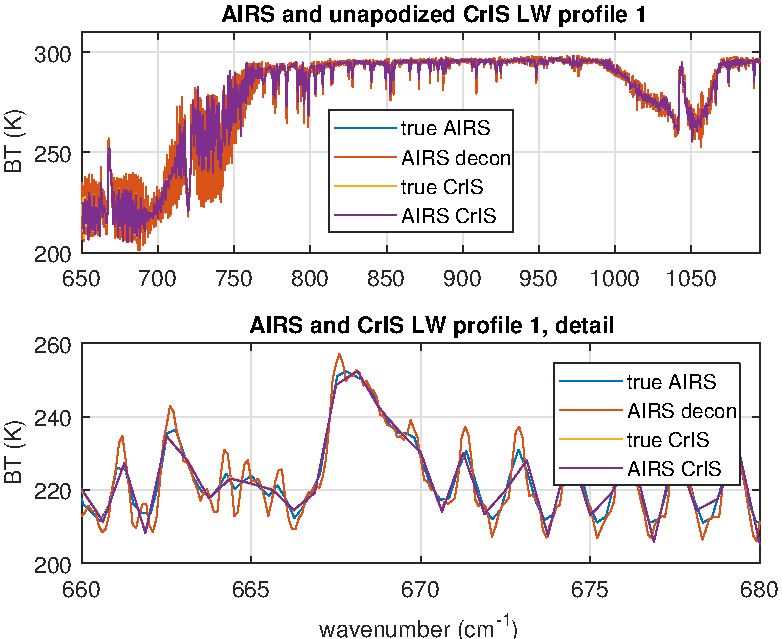
\includegraphics[height=7.5cm]{figures/a2cris_spec_LW.pdf}
%   \caption{true {\cris}, true {\airs}, deconvolved {\airs}, and
%     {\airs} {\cris}}
%   \label{specLW}
% \end{figure}

\begin{figure} % source a2cris_test1
  \centering
  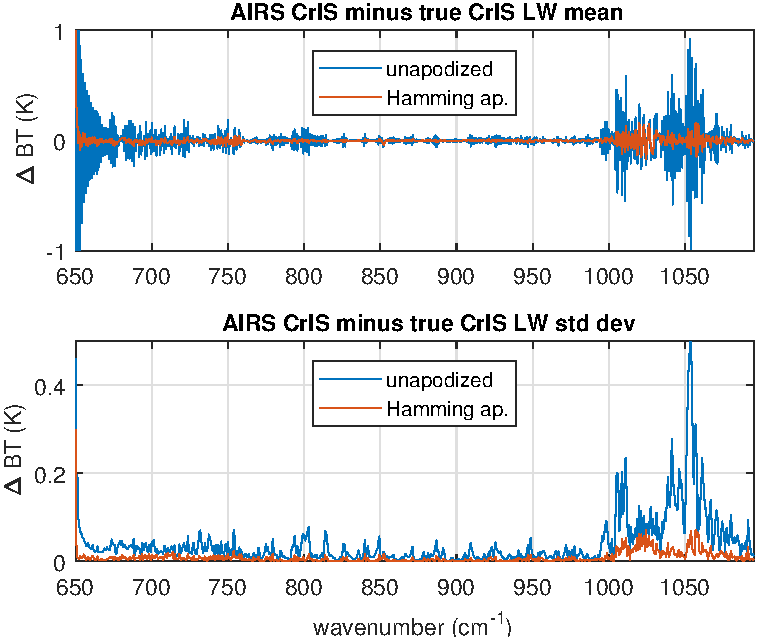
\includegraphics[height=7.5cm]{figures/a2cris_diff_LW.pdf}
  \caption{Mean and standard deviation of unapodized and Hamming
    apodized {\airs} {\cris} minus true {\cris}, for the {\cris} LW
    band}
  \label{diffLW}
\end{figure}

\begin{figure} % source a2cris_test1
  \centering
  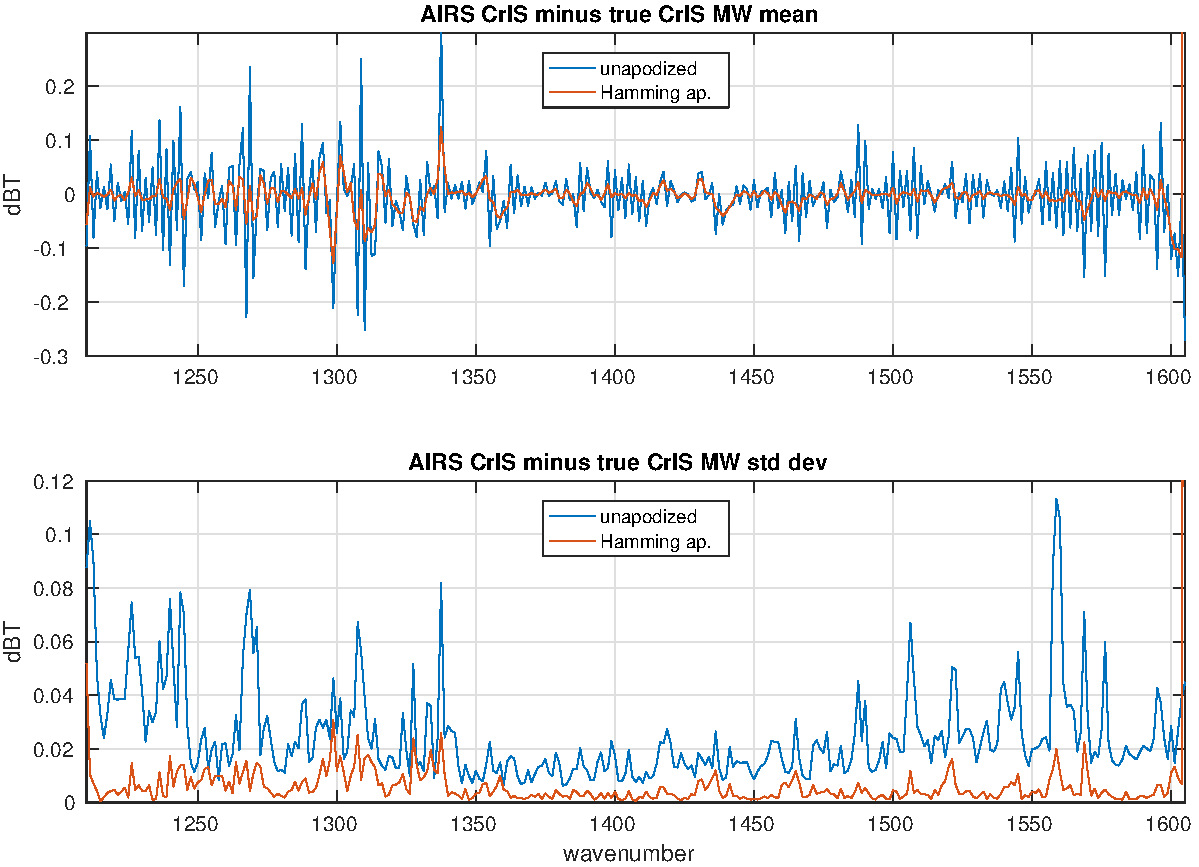
\includegraphics[height=7.5cm]{figures/a2cris_diff_MW.pdf}
  \caption{Mean and standard deviation of unapodized and Hamming
    apodized {\airs} {\cris} minus true {\cris}, for the {\cris} MW
    band}
  \label{diffMW}
\end{figure}

\begin{figure} % source a2cris_test1
  \centering
  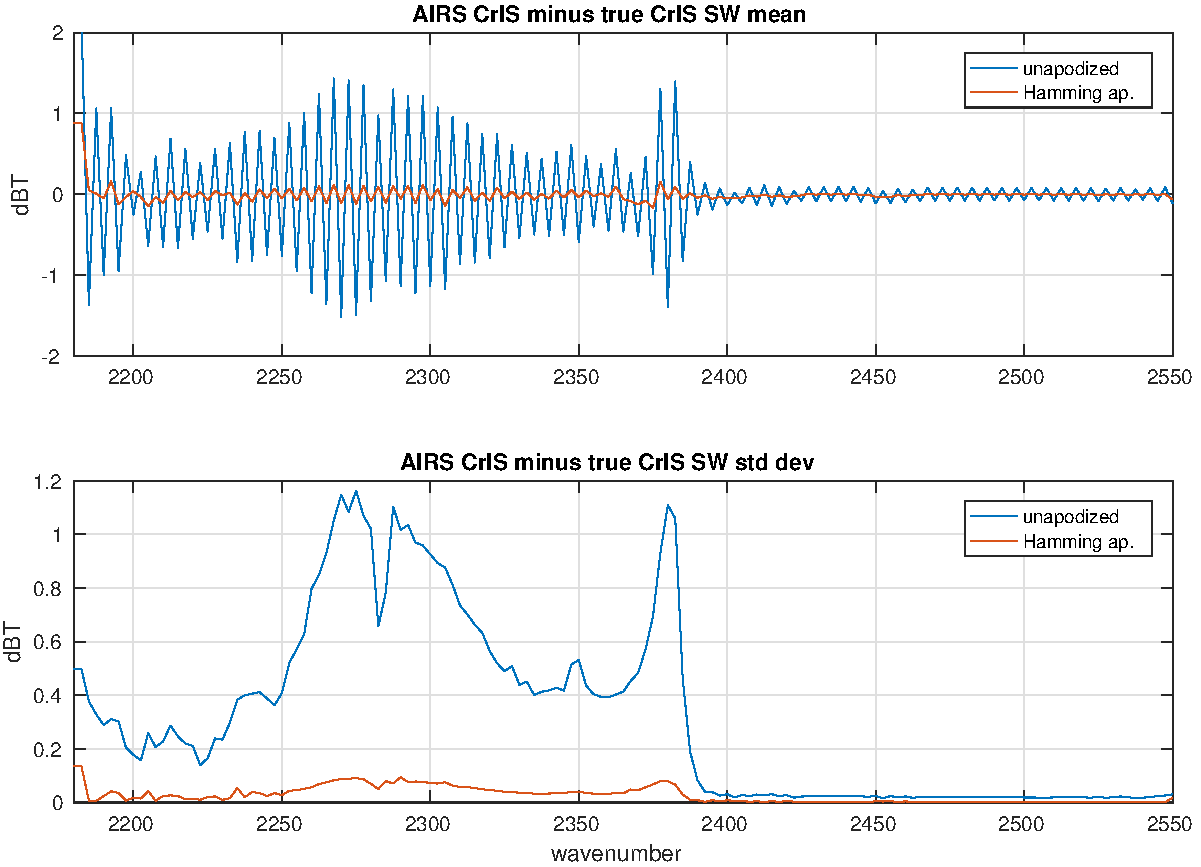
\includegraphics[height=7.5cm]{figures/a2cris_diff_SW.pdf}
  \caption{Mean and standard deviation of unapodized and Hamming
    apodized {\airs} {\cris} minus true {\cris}, for the {\cris} SW
    band}
  \label{diffSW}
\end{figure}

\begin{figure} % source a2cris_plot1.m
  \centering
  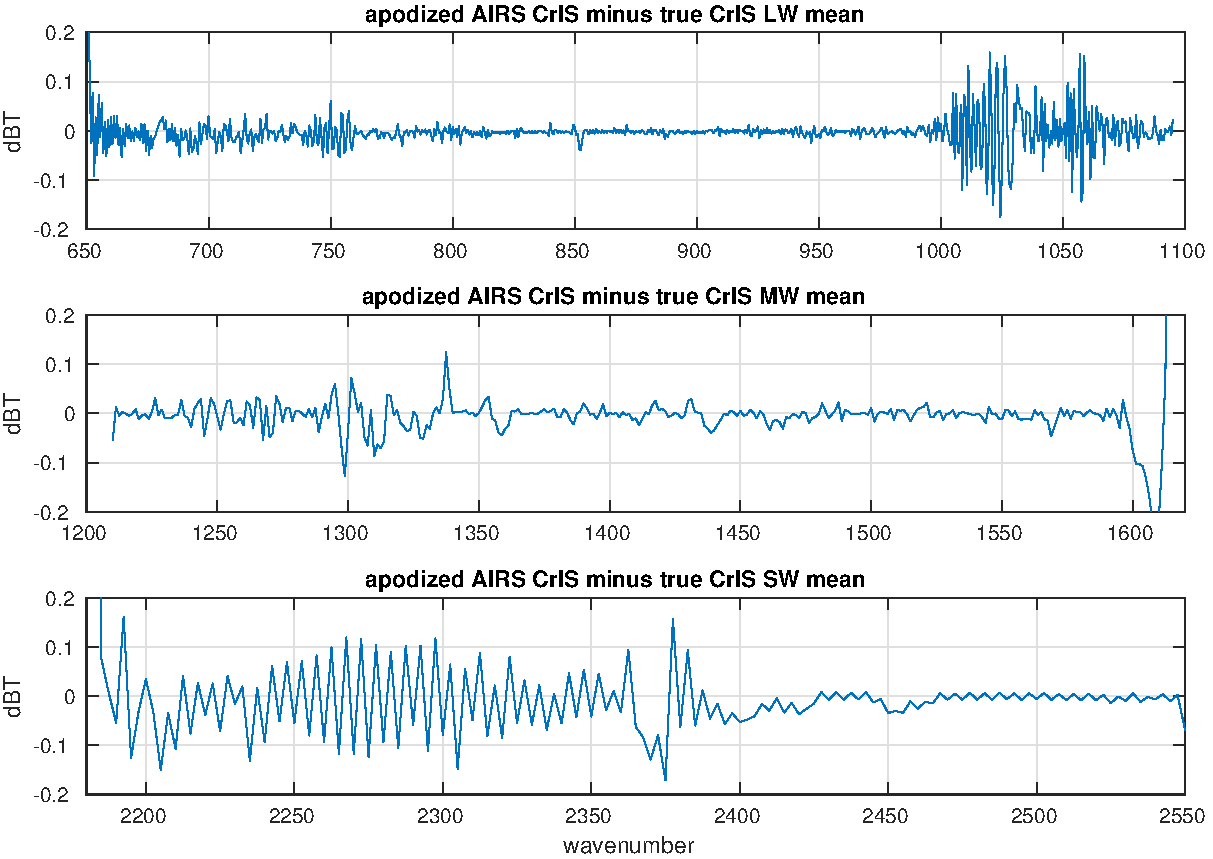
\includegraphics[height=7.5cm]{figures/combo_ap_dif_mean.pdf}
  \caption{Mean of apodized residuals for all three {\cris} bands}
  \label{meanAll}
\end{figure}

\begin{figure} % source a2cris_plot1.m
  \centering
  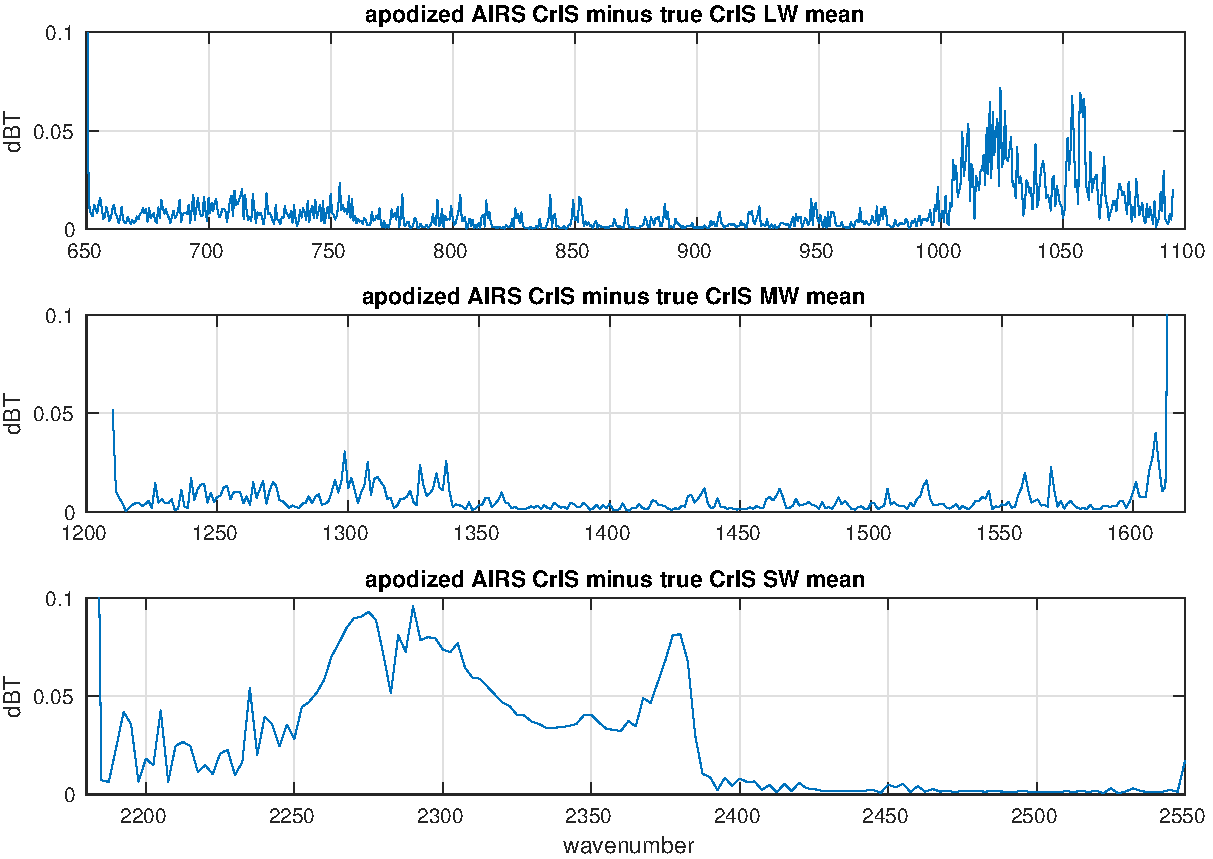
\includegraphics[height=7.5cm]{figures/combo_ap_dif_std.pdf}
  \caption{Standard deviation of apodized residuals for all three
    {\cris} bands}
  \label{stdAll}
\end{figure}

\begin{figure} % source a2cris_test1
  \centering
  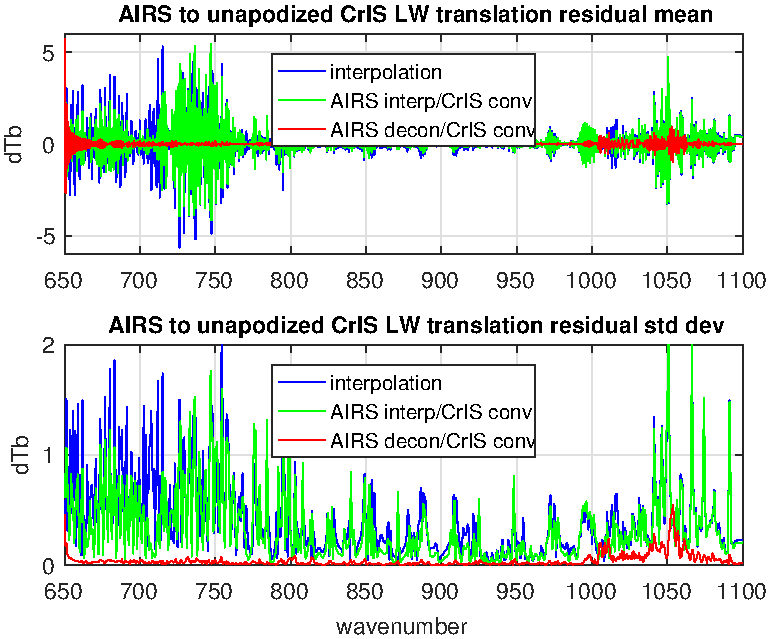
\includegraphics[height=7.5cm]{figures/a2cris_interp_LW.pdf}
  \caption{spline interpolation, interpolation with convolution, 
    and deconvolution with convolution for the {\cris} LW band}
  \label{intpLW}
\end{figure}

Deconvolution is significantly better than interpolation for the
{\airs} to {\cris} translation.  We consider two cases.  For the
first, start with true {\airs} and interpolate radiances directly 
to the {\cris} user grid with a cubic spline.  For the second,
interpolate true {\airs} to the 0.1 {\wn} intermediate grid with a
cubic spline and then convolve this to the use {\cris} user grid.
Figure~\ref{intpLW} shows interpolated {\cris} minus true {\cris}
for the LW band, without apodization.  The two-step interpolation
works a little better than the simple spline, but both residuals are
significantly larger than for the translation with deconvolution.
Results for the MW are similar, while the unapodized comparison is
less clear for the SW.  With Hamming apodization, the residuals with
deconvolution are significantly less than interpolation for all
three bands.

Residuals for the {\airs} to apodized {\cris} translation are
already small, and have no significant DC bias.  But there is some
regularity in the residual, including an oscillation with period two
channel steps.  We show that a linear correction can significantly
reduce this residual.  This is a standard technique but worth
describing briefly because the reduction is significant.

For these tests we start with kcarta radiances calculated from a 
set of 7377 radiances calculated from mostly cloudy AIRS profiles.
spanning several consecutive days.  These are split randomly into
dependent and independent sets.  Bias or regression coefficients are
taken from the dependent set, and tests are done on the independent
set.  As with the 49 profile set ``true {\airs}'' channel radiances
are calculated by convolving with {\airs} SRFs and ``true {\cris}''
by convolving to the {\cris} instrument specifications.

Note the difference in statistical approaches here and in section
\ref{airs2cris}.  There we used a small, largely uncorrelated set of
49 profiles chosen to span all common clear atmospheric conditions,
and intended for developing and testing radiative transfer codes.
For the statistical correction we use a more typical mix of clear
and cloudy data spanning several days, moderately correlated, and
large enough to allow for partition into significant dependent and
independent sets.

Figure \ref{statLW} is a comparison of bias, linear, and quadratic
corrections for a representative dependend/independent partition.
The residuals vary with the partition but the standard deviation is
consistently significantly less for the linear and quadratic cases.
The linear and quadratic corrections are nearly identical, the
quadratic coefficient is very close to zero.  Figure \ref{coefLW}
shows the weights for the linear fits shown above.  The $a$ weight
is very close to 1 and the $b$ weight to earlier bias values.

Figures \ref{statMW} and \ref{statSW} show the linear correction 
is giving a similar significant improvement in the MW standard
deviation in comparison with the LW, and a small improvement in the
SW.  As in the LW the mean residuals vary significantly depending on
the dependent/independent partition, but the standard deviations are
relatively stable.

\begin{figure} % source a2cris_stat4.m
  \centering
  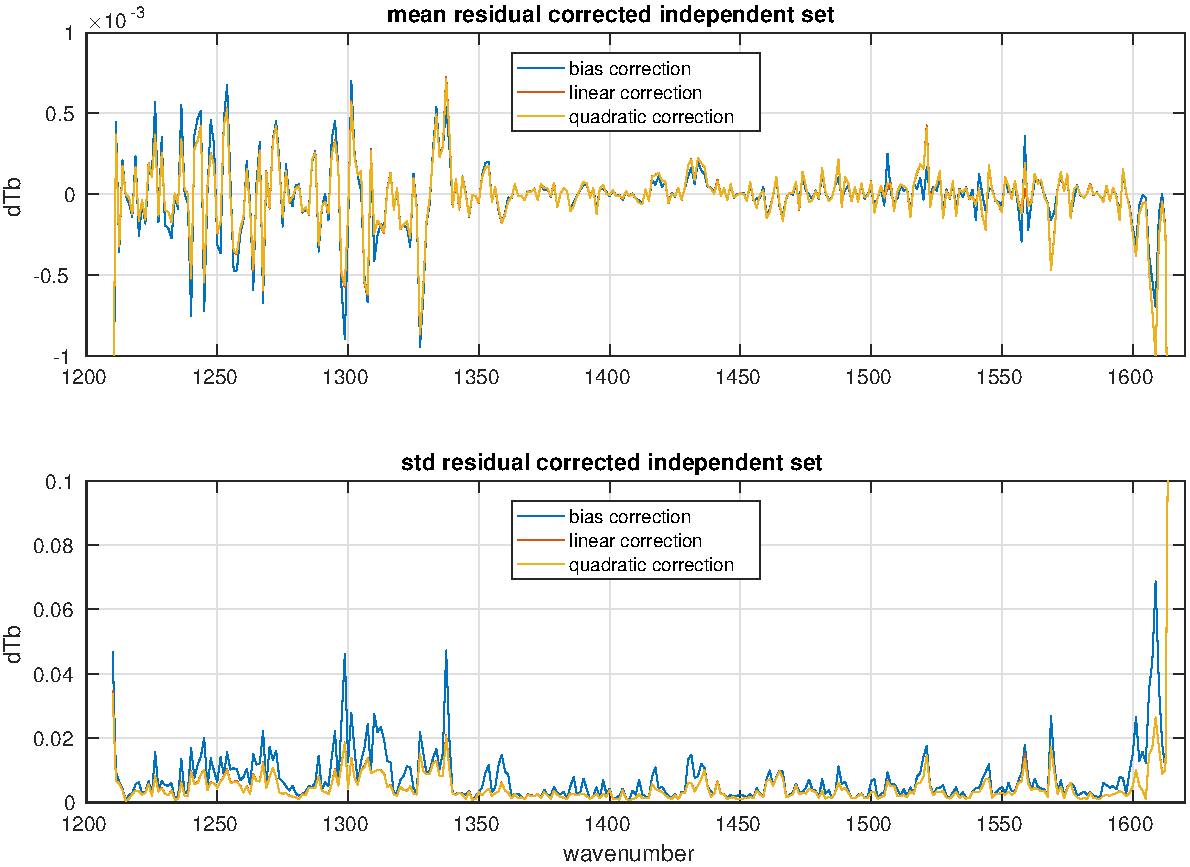
\includegraphics[height=7.5cm]{figures/a2cris_stat_LW.pdf}
  \caption{Mean and standard deviation of LW corrected apodized
    residuals for the independent subset of the 7377 profile set}
  \label{statLW}
\end{figure}

\begin{figure} % source a2cris_stat4.m
  \centering
  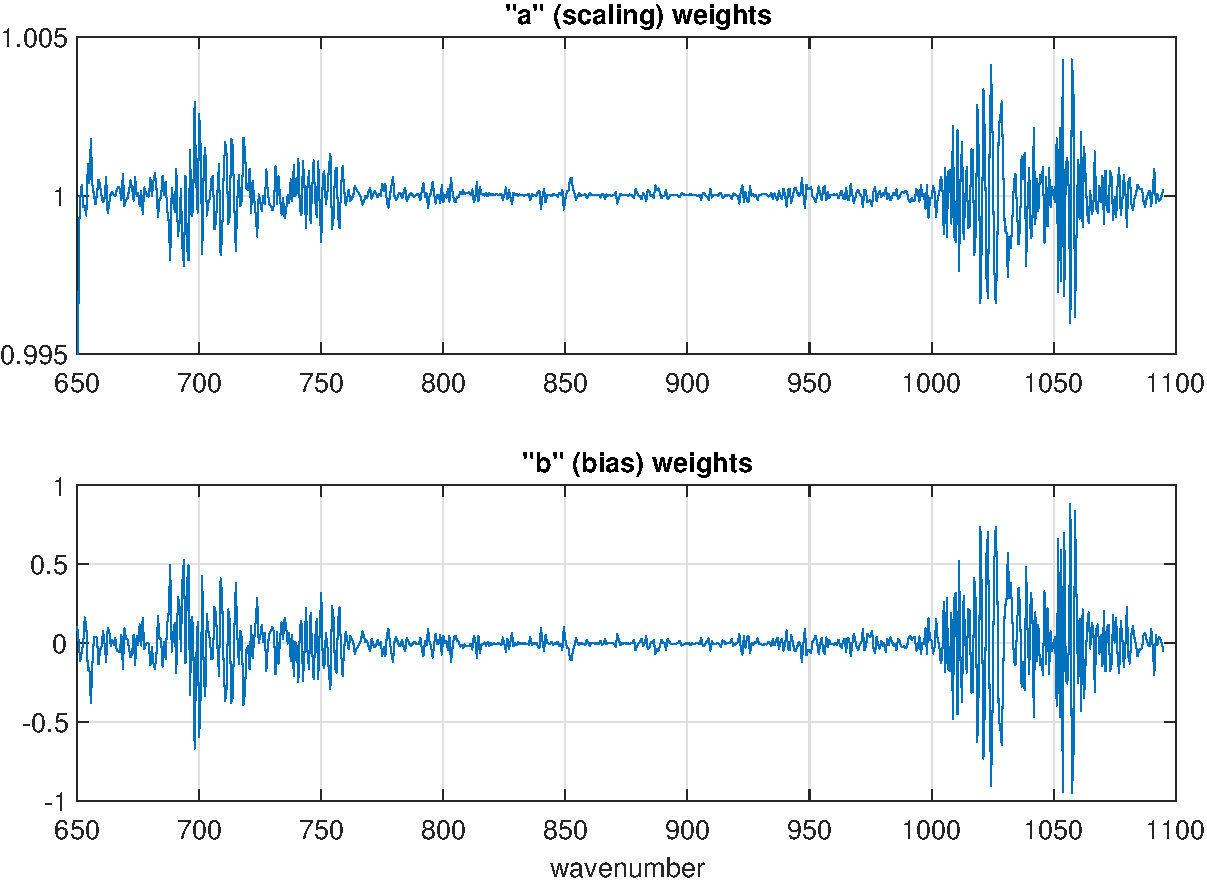
\includegraphics[height=7.5cm]{figures/a2cris_coef_LW.pdf}
  \caption{LW $a$ and $b$ weights for the linear correction $ax+b$}
  \label{coefLW}
\end{figure}

\begin{figure} % source a2cris_stat4.m
  \centering
  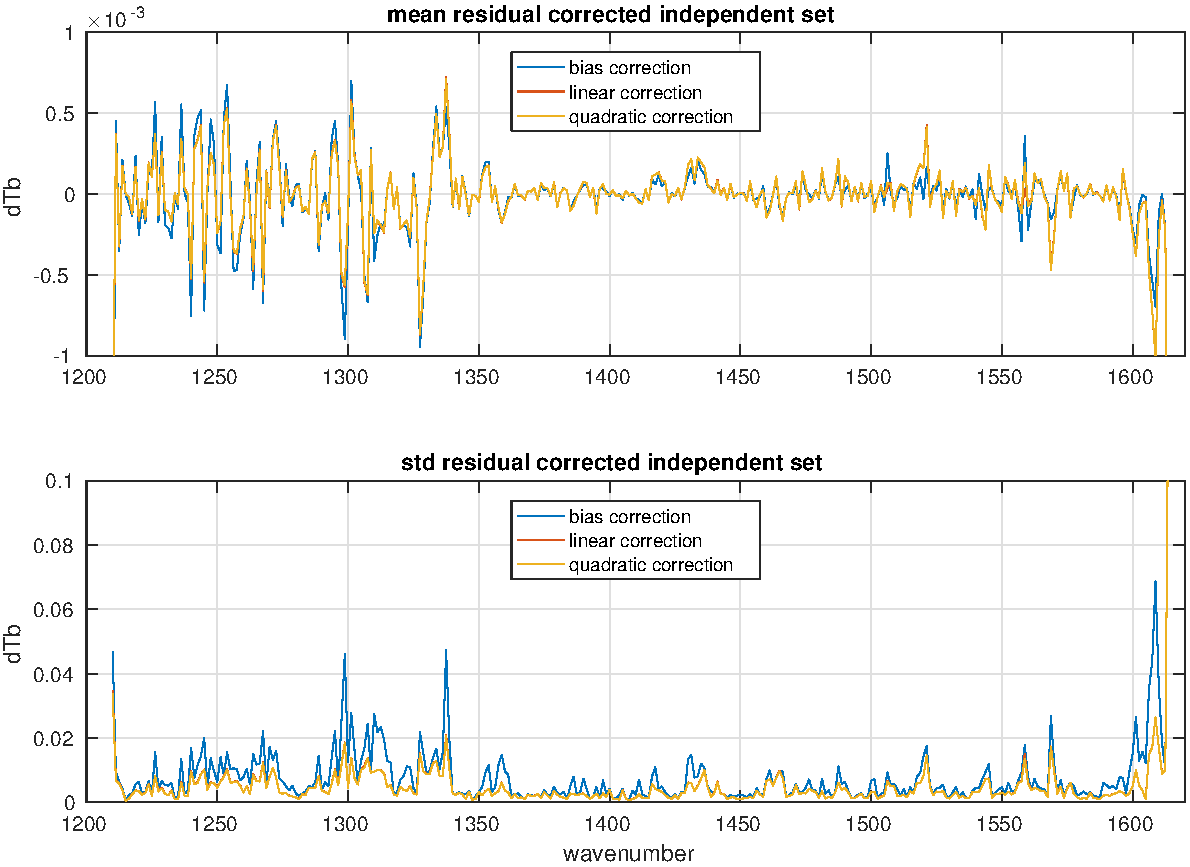
\includegraphics[height=7.5cm]{figures/a2cris_stat_MW.pdf}
  \caption{Mean and standard deviation of MW corrected apodized
    residuals for the independent subset of the 7377 profile set}
  \label{statMW}
\end{figure}

\begin{figure} % source a2cris_stat4.m
  \centering
  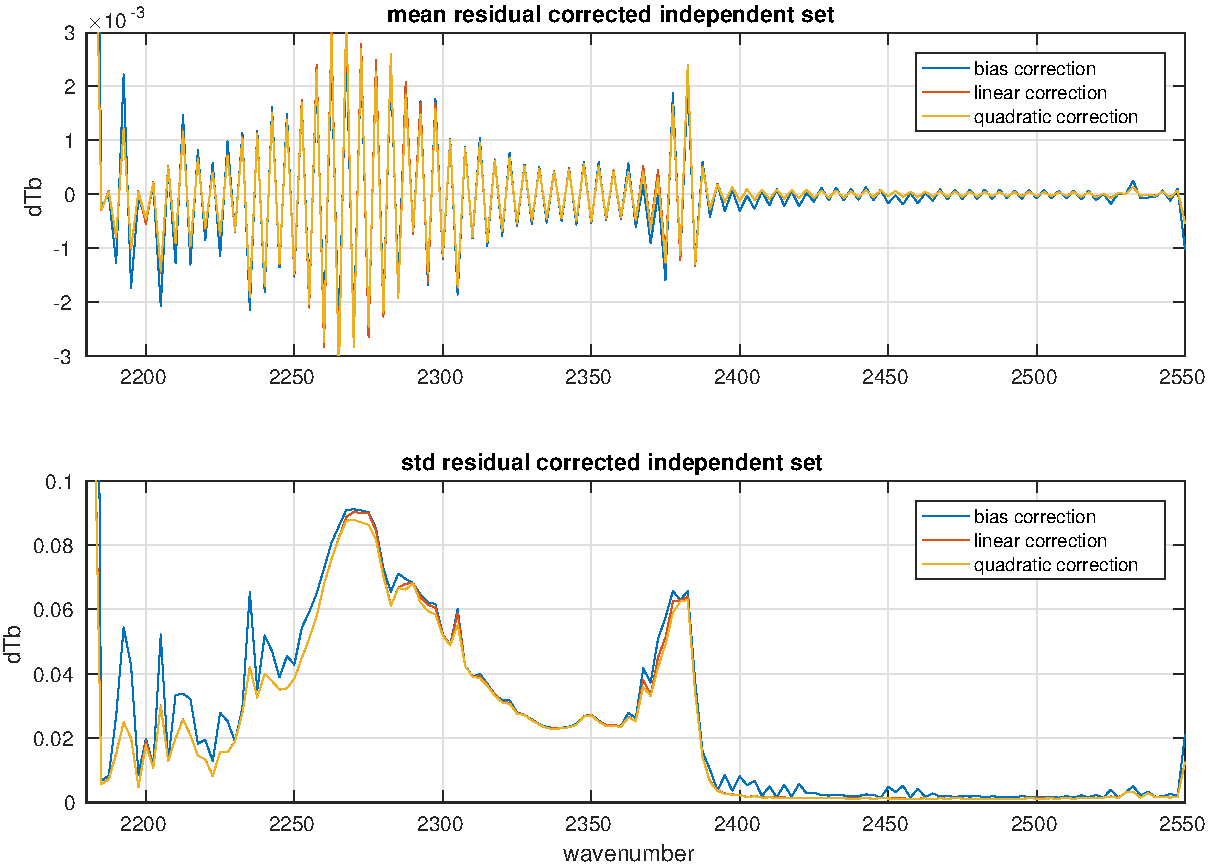
\includegraphics[height=7.5cm]{figures/a2cris_stat_SW.pdf}
  \caption{Mean and standard deviation of SW corrected apodized
    residuals for the independent subset of the 7377 profile set}
  \label{statSW}
\end{figure}

% \FloatBarrier
% \section{Deconvolution to constant resolving power}
% \label{airsL1d}
% 
% Section \ref{decon} raised the question of the inherent resolution
% of the deconvolution.  There we compared the deconvolution (without
% reconvolution) to calculated radiances with an oversampled resolving
% power of 2000.  But the residual was quite large.  
% 
% Similar to the situation with convolution to the {\cris} user grid,
% 

\FloatBarrier
\section{Alternate Translations}
\label{alttrans}

In the remainder of this section we consider reconvolution to
idealized grating instruments with resolving power of 1200 and 700.
Define an {\airs} L1d basis with the generalized Gaussian response
function above, with $\fwhm = v / \hbox{resolving power}$ and $dv =
\fwhm / 2$, and with the $dv$-spaced channel steps starting at
$v_0$.  In contrast with the regular spacing used for the {0.1~\wn}
intermediate grid, this is not oversampled.

% For this and similar comparisons both the reference truth (``true
% L1d'') and the reconvolution targer (L1c to L1d) are done using the
% same L1d channel sets--that is, sets with the same resolving power
% and starting channel.  

Figure \ref{L1d1200} shows residuals for reconvolution to an L1d
basis with resolving power of 1200, the nominal {\airs} resolution
and figure \ref{L1d700s} shows residuals for a resolving power of
700, half the best {\airs} resolving power of 1400 in the LW.  Note
the different x-axes in the two figures.  The uncorrected residuals
are for the deconvolution/reconvolution transform ``L1C to D'' minus
``true L1D'', Resolution is lost in shifting channel centers to a
single regular function of frequency.  The L1d residuals dependend
in part on the starting channel, and so on how the SRF peaks line up
with the L1c set.  The residuals above are the result of a rough fit
for $v_0$.  For a resolving power of 1200 this gave $v_0$ equal to
the first L1c channel, while for 700 it was the first L1c channel
plus $0.2$~\wn.

The residuals are reduced significantly with a linear correction.
This is discussed in more detail in the next section.  But the key
idea is to fit for a separate linear correction for each channel
using a large mostly cloudy dependent set, and then use the 49
profile fitting set---the same set we are using for most other tests
here---as the independent set.  The separate functions guarantee no
cross correlations are introduced, and the fitting profile test is
more strict than for example splitting the cloudy set into dependent
and independent sets, in the sense that the fitting profles are less
correlated and the residuals for the fitting set are larger.

% Note that convolution, deconvolution, and apodization are done
% with radiances while spectra are presented and statistics done
% after translation to brightness temperatures.

% The L1c to L1d translation can be represented as a single linear
% transform $S_d\cdot S_c^{-1}$, where $S_c$ and $S_d$ are the
% transforms taking the intermediate grid to L1c and L1d channels and
% $S_c^{-1}$ the pseudo-inverse of $S_c$.  We can get such a tranform
% in other ways, for example by regression to find $X$ that minimizes
% the residual $\|X r_c - r_d\|_2$ for L1c and L1d radiance sets $r_c$
% and $r_d$.  We consider this further in section \ref{alttrans}.

\begin{figure} % source L1d_regr1.m
  \centering
  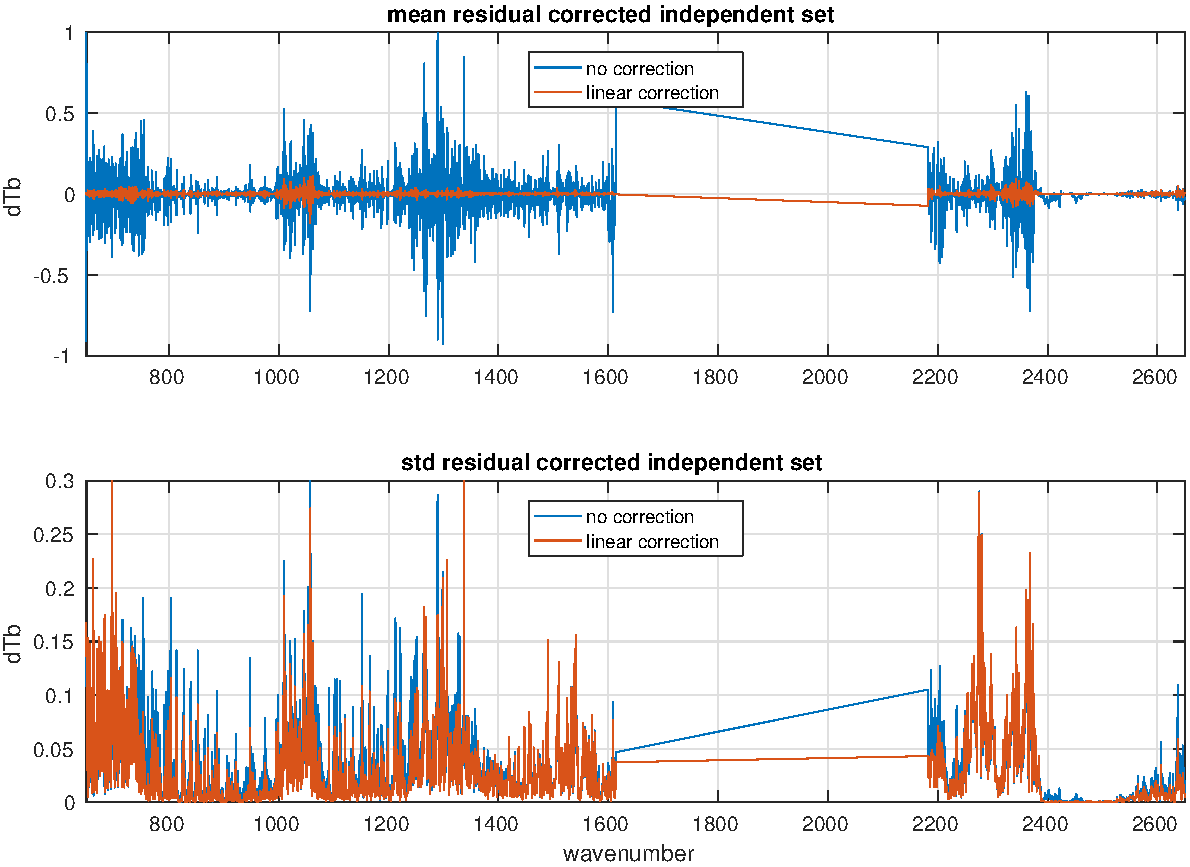
\includegraphics[height=7.5cm]{figures/L1d_corr_1200.pdf}
  \caption{mean and standard deviation over the 49 fitting profiles
    for the L1c to L1d translation minus true L1d for a resolving
    power of 1200}
  \label{L1d1200}
\end{figure}

\begin{figure} % source L1d_regr1.m
  \centering
  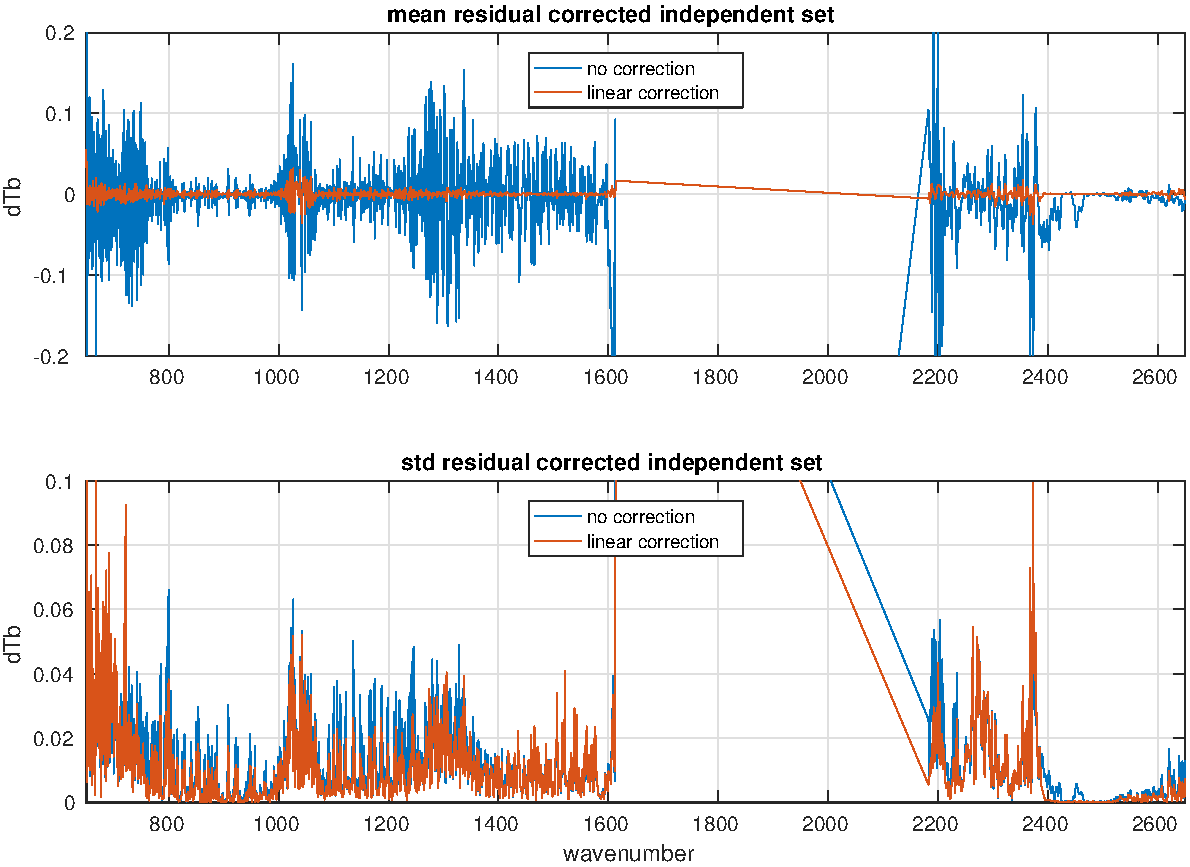
\includegraphics[height=7.5cm]{figures/L1d_corr_700.pdf}
  \caption{mean and standard deviation over the 49 fitting profiles
    for the L1c to L1d translation minus true L1d for a resolving
    power of 1200}
  \label{L1d700s}
\end{figure}

The L1c to L1d translation can be represented as a single linear
transform $S_d\cdot S_c^{-1}$, where $S_c$ and $S_d$ are the
transforms taking the intermediate grid to L1c and L1d channels and
$S_c^{-1}$ the pseudo-inverse of $S_c$, that is, the deconvolution
transform.  We can get such a tranform in other ways, for example by
regression to find $X$ that minimizes the residual $\|X r_c -
r_d\|_2$ for L1c and L1d radiance sets $r_c$ and $r_d$.  If $r_c$ and
$r_d$ are $m$ and $n$ by $k$ matrices, then if $k <= m$ we can simply
solve for $X$.  If $k < m$ the system is underdetermined; in this
case the residual is zero but extrapolation behavior is typically
poor.  If $k > m$ we can find $X$ by regression, and extrapolation
behavior can be quite good if we regress against large sets of
representative data.  In practice this seems to work very well, at
least for minimizing both dependent and independent set residuals.
But in contrast with the sharply banded composite transform $S_d\cdot
S_c^{-1}$ the resulting transform is full of unexpected correlations
and so may not be suitable for applications where we want to trace
channel dependencies in the translation.

Despite the resolution loss, deconvolution is significantly better
than interpolation for the L1c to L1d translation.  We consider two
cases.  For the first, start with true L1c and interpolate radiances
directly to the L1d grid with a cubic spline.  For the second,
interpolate true L1c to the 0.1 {\wn} intermediate grid with a cubic
spline and convolve this to the L1d channel set.
Figure~\ref{interpL1d} shows interpolated L1d minus true L1d.  The
two-step interpolation works a little better than the simple spline,
but is still much larger than the residual for translation with
deconvolution.

\begin{figure} % source L1d_test2.m
  \centering
  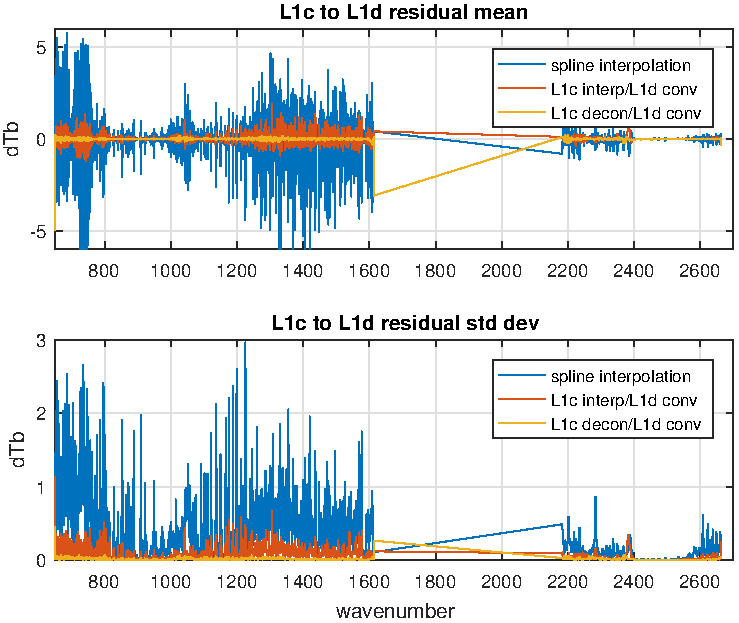
\includegraphics[height=7.5cm]{figures/CtoD_interp_diff.pdf}
  \caption{spline interpolation, interpolation with convolution, 
    and deconvolution with convolution for the {\airs} L1c to L1d
    translation with $v_0=649.822$~\wn\ and a resolving power of 700}
  \label{interpL1d}
\end{figure}

\FloatBarrier
\section{Applications and conclusions}
\label{appcon}

\FloatBarrier
\bibliographystyle{abbrv}
\bibliography{decon}

\end{document}

